\section{Analysis}\label{sec:analysis}

\subsection{TPC}

\subsubsection{$^{57}$Co S1 energy}
Fig.~\ref{fig:CalibData:Co57} shows a comparison of the scintillation signal S1 spectrum of a $^{57}$Co calibration source data deployed next to the cryostat and close to the TPC active volume center. Overlayed is the S1 distribution from an equivalent selection of G4DS MC simulation. Besides passing basic cuts like baseline found or all electronics channels present, the events were restricted to single-site interactions having one S1 and one S2 pulse, also the $^{39}$Ar background has been subtracted statistically. In the MC instead of an electronics simulation a clustering algorithm has been applied, that groups individual energy deposits and sums up the corresponding number of PE. A single-cluster cut has been applied to correspond to single-site interactions. The $^{57}$Co gamma ray spectrum (122 keV) reaching the TPC is significantly distorted by having to pass through the stainless steel source holder, outer and inner cryostat and the copper field cage rings before reaching the TPC's active volume.  These effects are accounted for by the MC even though refinements in the material description will further improve the already encouraging data-MC agreement. 

\begin{figure}[htbp]
\centering
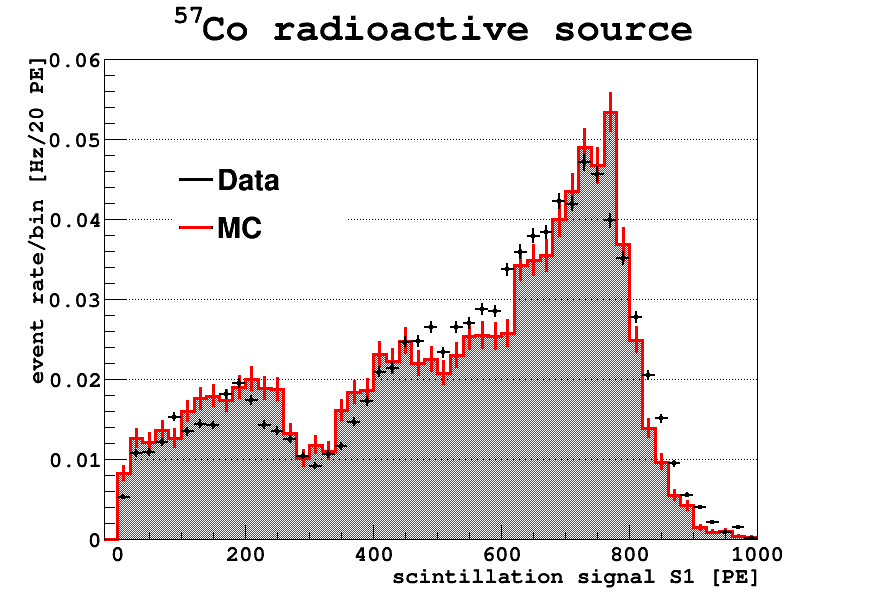
\includegraphics[width=0.6\textwidth]{./Figures/Co57_LArTPC_center.png}
\caption{Data-MC comparison for the $^{57}$Co source deployed next to the cryostat. While some improvements are yet to be made, the level of agreement between the simulation and the various complex features of the data is very encouraging.
%A lack of resolution in the MC is expected as smearing due to electronics and reconstruction effects are not taken into account in the MC. THIS DOES NOT MAKE SENSE
\label{fig:CalibData:Co57}}
 \end{figure}


\subsubsection{position distributions}
\begin{figure}[htbp]
\centering
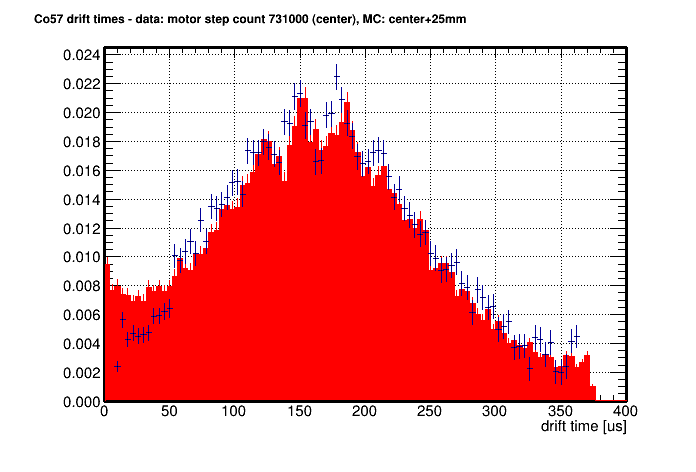
\includegraphics[width=0.55\textwidth]{./Figures/Co57_tdrift_data_731000-center+25mm.png}
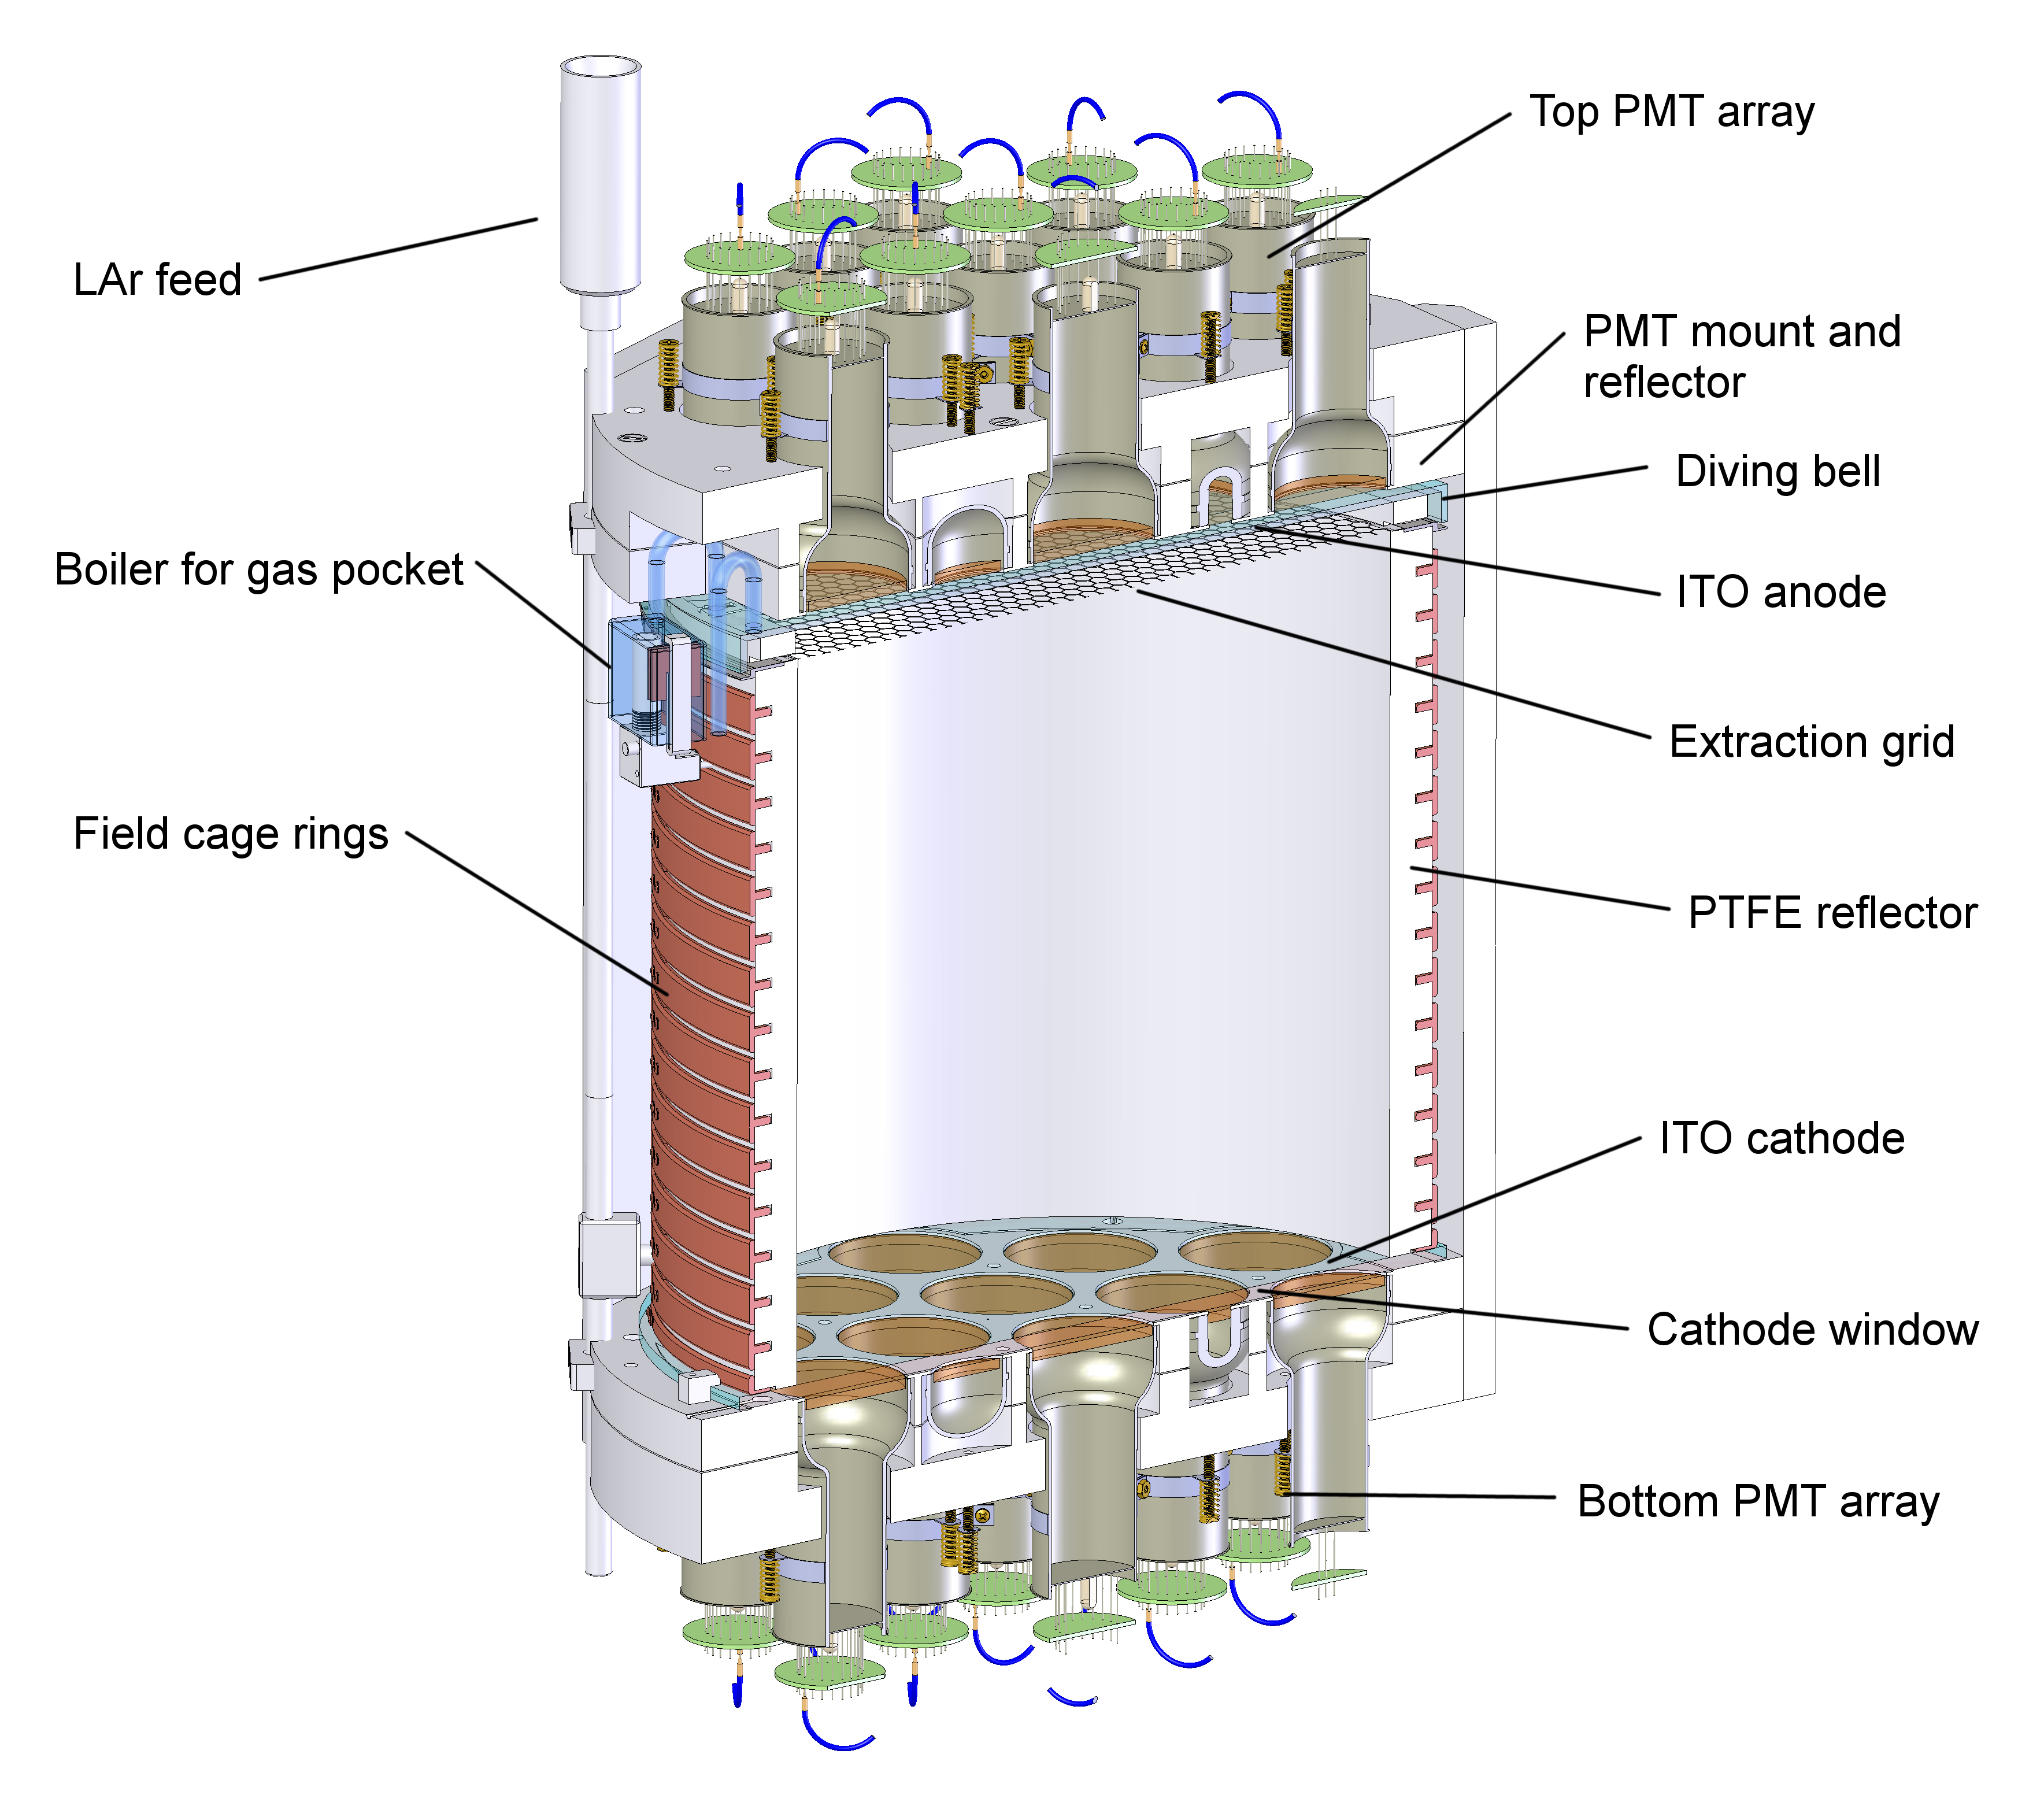
\includegraphics[width=0.43\textwidth]{./Figures/50kg_Assembly_4-1-13_section_annotated_2.JPG}
\caption{\textit{left}: Data-MC comparison for the t$_{drift}$ distribution of the $^{57}$Co source deployed next to the cryostat and close to the active volume center. 
\textit{right:} Schematics of the TPC (without inner and outer cryostat) showing in particular the field rings, that cause a characteristic wave in the t$_{drift}$ spectrum of $^{57}$Co, which is also reproduced in MC (left) \cite{DS50:first_paper}.
\label{fig:CalibData:Co57:t_drift}}
\end{figure}

The t$_{drift}$ distribution of $^{57}$Co in Fig.~\ref{fig:CalibData:Co57:t_drift} is the same run set and event selection as for the S1 spectrum in Fig.~\ref{fig:CalibData:Co57}. It nicely illustrates the impact that the field rings have on the distribution. Fig.~\ref{fig:CalibData:XY_distrib} shows XY distributions of $^{133}$Ba and $^{137}$Cs sources deployed touching the cryostat from the left and right, respectively, exemplarily out of a pool of possible XY distributions.

\begin{figure}[htbp]
\centering
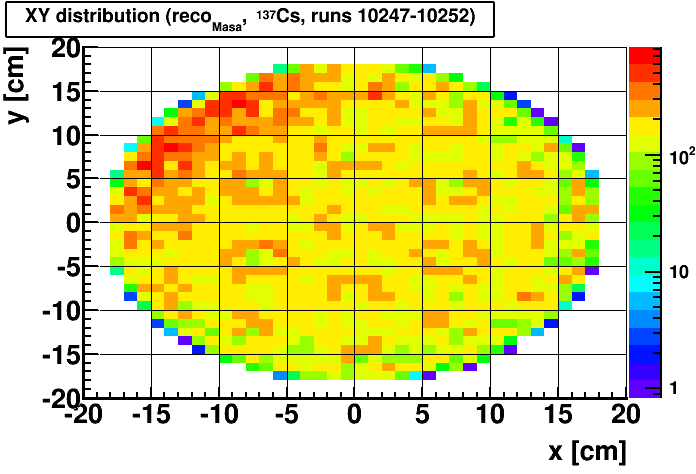
\includegraphics[width=0.55\textwidth]{./Figures/XY_Cs137_200Vcm_run10247_10252.png}
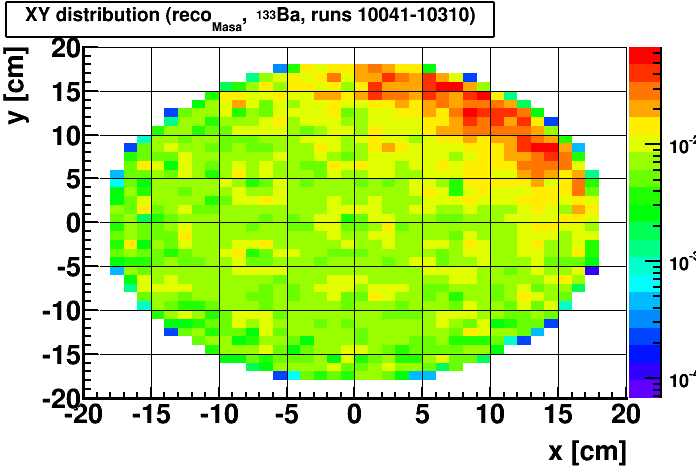
\includegraphics[width=0.43\textwidth]{./Figures/XY_Ba133_driftHV200_run10041_10310_right.png}
\caption{Two examples of XY distributions of $^{137}$Cs (left) and $^{133}$Ba (right) calibration source runs with the sources touching the cryostat from the left ($^{137}$Cs) and right ($^{133}$Ba). The $^{39}$Ar background is not subtracted and fills the TPC uniformly.
\label{fig:CalibData:XY_distrib}}
\end{figure}



\subsubsection{$^{241}$Am$^9$Be neutron data}\label{sec:CalibData:NR}

\begin{figure}[htbp]
\centering
\subfigure{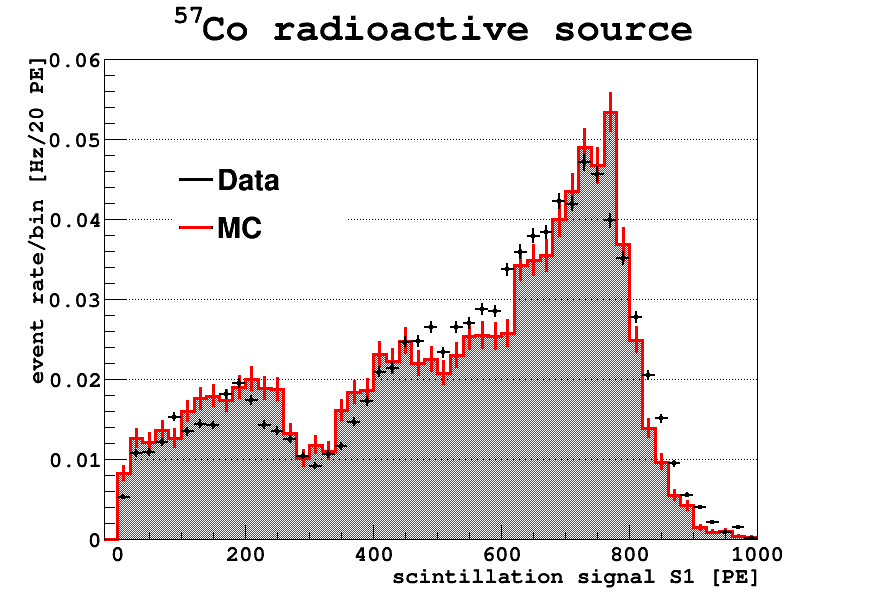
\includegraphics[width=0.51\textwidth]{./Figures/Co57_LArTPC_center.png}}
%\subfigure{\includegraphics[width=0.46\textwidth]{./Figures/F90_data_DocDB1075.png}}
\subfigure{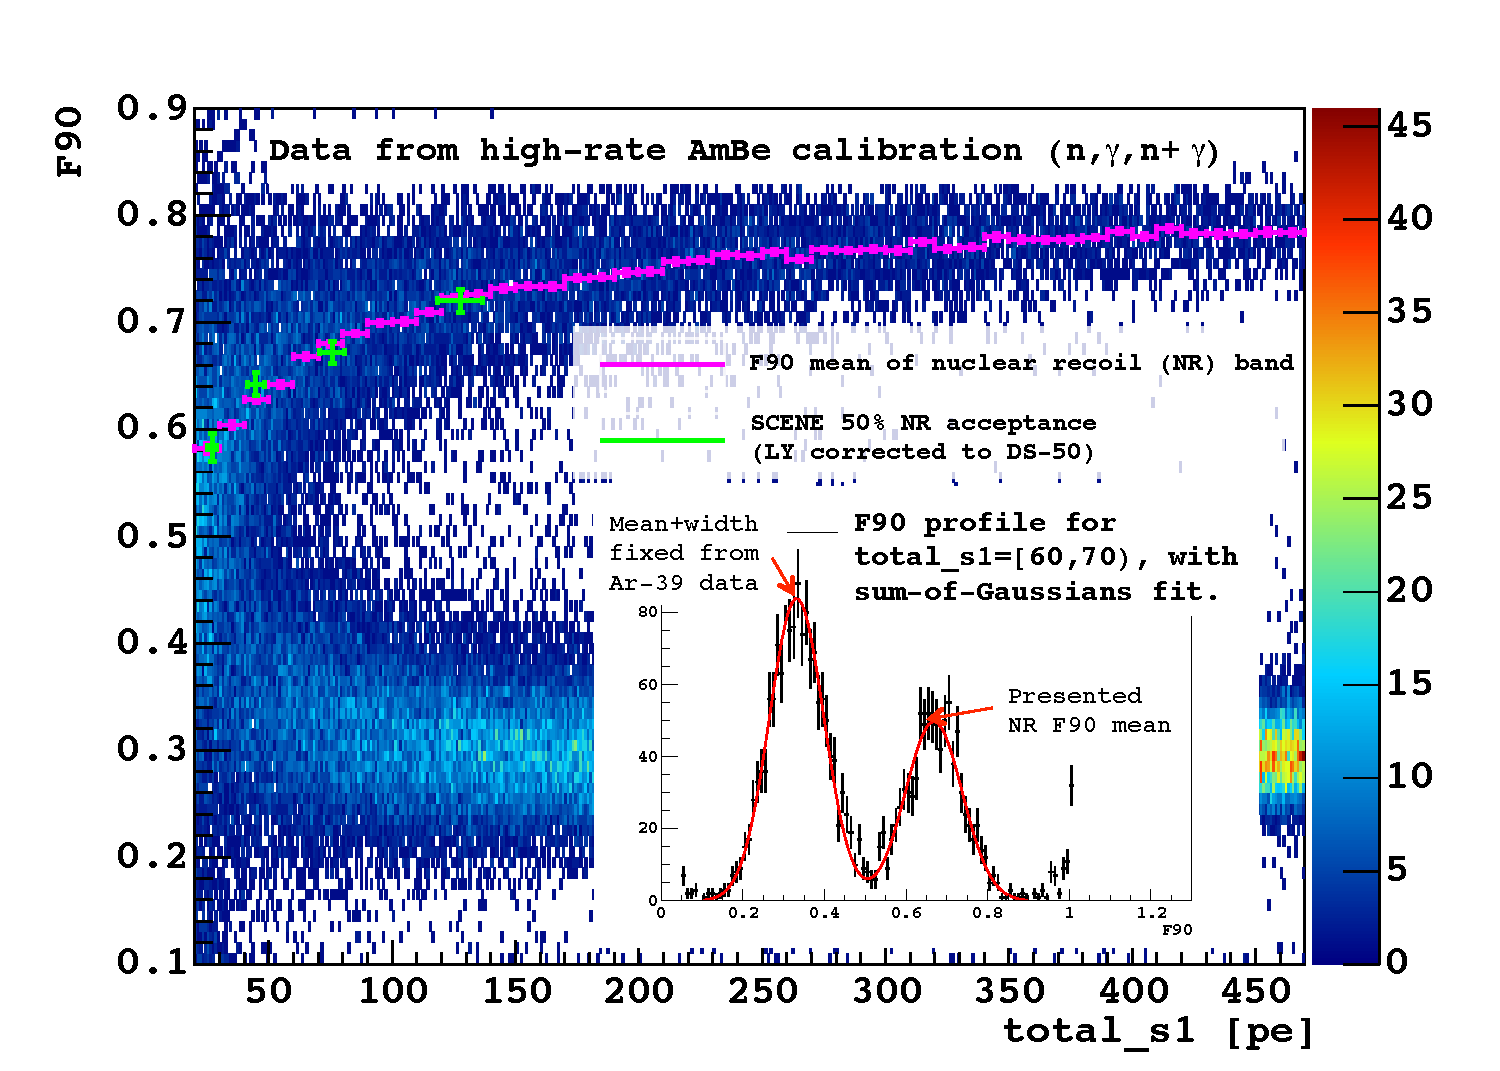
\includegraphics[width=0.47\textwidth]{./Figures/nr_f90_fit_apr2015_v8.pdf}}
 \caption{\textit{left}: Data-MC comparison for the $^{57}$Co source deployed next to the cryostat. While some improvements are yet to be made, the level of agreement between the simulation and the various complex features of the data is very encouraging.
%A lack of resolution in the MC is expected as smearing due to electronics and reconstruction effects are not taken into account in the MC. THIS DOES NOT MAKE SENSE
%\textit{right}: Distribution of pulse shape discrimination parameter F90 vs.~ S1 from \ar\ in AAr, overlayed with calibration data from $^{57}$Co and $^{133}$Ba sources. Good agreement with  the internal $^{39}$Ar illustrates the consistency of the calibration data.
\textit{right:} Plot of F90 vs. scintillation signal S1 from a high rate AmBe neutron source calibration of \dsf.  The pink line shows the mean F90 for the nuclear recoil band, while the points in green show the F90 values scaled from SCENE measurements and used in our publication Ref.~\cite{ds:ds-50-PLB}. There is very good agreement between the two.  The high source intensity and correlated neutrons and $\gamma$-ray emission by the AmBe source contribute events outside the nuclear recoil and electron recoil bands. 
\label{fig:CalibData:F90}}
 \end{figure}


%Distributions of the F90 pulse shape parameter from $^{57}$Co and $^{133}$Ba gamma sources outside the LAr-TPC are in good agreement with those from the internal calibration provided by the \ar \, decays, demonstrating the good quality of the calibration data set (Fig.~\ref{fig:CalibData:F90}, right). 

%At the time of publication of our paper Ref. \cite{ds:ds-50-PLB},  neutron calibration data was not available.  Therefore the WIMP search box for nuclear recoils was set based on measurements of F90 in the SCENE experiment \cite{scene2}. Now, a preliminary analyses of AmBe neutron source exposures shown in Fig.~\ref{fig:CalibData:F90}, lower left proves the good agreement between the extrapolated SCENE results and actual \dsf\ data.  

The WIMP search box and nuclear recoil acceptance in our paper~\cite{ds:ds-50-PLB} were established
without the availability of neutron calibration data in \dsf.  
The mean F90 from the ScENE experiment~\cite{scene2} was scaled to the light yield of DarkSide-50, and the electron and nuclear recoil acceptance curves were determined from an analytic statistical model of the F90 distributions as a function of energy. While we have full confidence in this approach, the 
data taken in the calibration campaign with the Am-Be neutron source now allow it to be directly
verified.  The mean F90 for nuclear recoils in \dsf\ is found to agree closely with the corresponding
scaled ScENE results, as shown in Fig.~\ref{fig:CalibData:F90}, right). 
%The same figure also shows Fig.~\ref{fig:CalibData:F90}, right also shows that the data with the Am-Be source will give us the mean F90 for nuclear recoils at energies beyond those measured by ScENE. 
(The higher-than-optimal intensity of this AmBe source and its 
correlated neutron and gamma ray emissions contribute events in the plot outside the nuclear recoil and electron recoil bands.)

\subsubsection{Z and XY of source position}
Tests at LNGS established the deployment system's positioning accuracy to be about $\pm$1 cm after a 7 meter journey into the DarkSide-50 detector.
%comment to the "about $\pm ": the tilde $~ \pm$ did not show up at all in the output.

 %Our first results show that the source can be positioned after its 7 meter journey into the DarkSide-50 detector with an accuracy of $~ \pm $1 cm.


This result is being validated using calibration campaign data in an ongoing analysis. 


\subsection{Liquid Scintillator Veto}\label{sec:LSV:gammasources}

In January and February 2015 the reconstitution of the LSV scintillator was completed and a second AmBe neutron source calibration of the LSV calibration was undertaken to further study the various
neutron detection channels in the LSV. With a borated scintillator, a critical aspect of the neutron detection efficiency is the capability to observe the \brbortenground\
capture branch leading to a \enbortengroundalpha\ $\alpha$ + $^7$Li(g.s.) without the accompanying 478 keV $\gamma$-ray. Veto results are described in further detail below in Sec.~\ref{sec:veto}.



\subsection{Impact of Calibration Source Deployment on Stability and Radioactivity in LY}